%%%%%%%%%%%%%%%%%%%%%%%%%%%%%%%%%%%%%%%%%%%%%%%%%%%%%%%%%%%%%%%%%%%%%%
% Template Source: Dave Richeson (divisbyzero.com), Dickinson College
% Author: Louis Dod (13bytes.de)
%%%%%%%%%%%%%%%%%%%%%%%%%%%%%%%%%%%%%%%%%%%%%%%%%%%%%%%%%%%%%%%%%%%%%%
% Please report any errors either via pull request, issue (https://github.com/13Bytes/Uni-Merkzettel) or mail (coding@13bytes.de)
% Improvements are also gladly accepted
%%%%%%%%%%%%%%%%%%%%%%%%%%%%%%%%%%%%%%%%%%%%%%%%%%%%%%%%%%%%%%%%%%%%%%


\documentclass[a4paper,10pt,landscape]{article}
\usepackage{fontspec}
\usepackage[T1,EU1]{fontenc}
\usepackage{lmodern}    % font
\usepackage[frenchb]{babel} 
\usepackage{amssymb,amsmath,amsthm,amsfonts}
\usepackage{multicol,multirow}
\usepackage{calc}
\usepackage{ifthen}
\usepackage{mathrsfs}
\usepackage[landscape]{geometry}
\usepackage[colorlinks=true,citecolor=blue,linkcolor=blue]{hyperref}
\usepackage[colorinlistoftodos, ngerman]{todonotes}
\usepackage{xcolor,soul}
\usepackage{cancel}
\usepackage{multirow}
\usepackage{mathabx}
\definecolor{lime}{RGB}{51, 204, 51}
\definecolor{neptune}{RGB}{131,194,188}

\ifthenelse{\lengthtest { \paperwidth = 11in}}
    { \geometry{top=0.5in,left=.5in,right=.5in,bottom=.5in} }
	{\ifthenelse{ \lengthtest{ \paperwidth = 297mm}}
		{\geometry{top=.5cm,left=1cm,right=1cm,bottom=.5cm} }
		{\geometry{top=.2cm,left=1cm,right=1cm,bottom=.2cm} }
	}
\pagestyle{empty}
\makeatletter
\renewcommand{\section}{\@startsection{section}{1}{0mm}%
                                {-1ex plus -.5ex minus -.2ex}%
                                {0.5ex plus .2ex}%x
                                {\normalfont\large\bfseries}}
\renewcommand{\subsection}{\@startsection{subsection}{2}{0mm}%
                                {-1explus -.5ex minus -.2ex}%
                                {0.5ex plus .2ex}%
                                {\normalfont\normalsize\bfseries}}
\renewcommand{\subsubsection}{\@startsection{subsubsection}{3}{0mm}%
                                {-1ex plus -.5ex minus -.2ex}%
                                {1ex plus .2ex}%
                                {\normalfont\small\bfseries}}
                                
\newcommand{\OK}{\fcolorbox{black}{lime}{\rule{0pt}{1pt}\rule{1pt}{0pt}}}
\newcommand{\YO}{\fcolorbox{black}{blue}{\rule{0pt}{1pt}\rule{1pt}{0pt}}}
\newcommand{\NO}{\fcolorbox{black}{red}{\rule{0pt}{1pt}\rule{1pt}{0pt}}}
\DeclareRobustCommand{\hlcy}[1]{{\sethlcolor{cyan}\hl{#1}}}
\DeclareRobustCommand{\hlgr}[1]{{\sethlcolor{green}\hl{#1}}}
\newcommand{\NDTIME}{\textrm{\textcolor{yellow}{D}\textcolor{orange}{N}TIME}}
\newcommand{\NDSPACE}{\textrm{\textcolor{yellow}{D}\textcolor{orange}{N}SPACE}}
\newcommand{\bbZ}{\mathbb{Z}}
\newcommand{\bbP}{\mathbb{P}}
\newcommand{\bbV}{\mathbb{V}}
\newcommand{\bbE}{\mathbb{E}}
\newcommand{\x}{\underline{x}}
\newcommand{\om}{\underline{\omega}}
                
\makeatother
\setcounter{secnumdepth}{0}
\setlength{\parindent}{0pt}
\setlength{\parskip}{0pt plus 0.5ex}
% -----------------------------------------------------------------------
\begin{document}

\raggedright
\footnotesize

Detection- \& Patternrecognition - Matr.: \hspace{3cm} Name: \hspace{16cm}
{\tiny{\href{https://github.com/13Bytes/Uni-Merkzettel}{\textcolor{gray}{github.com/13Bytes/Uni-Merkzettel}}}}\\

\begin{multicols}{3}
    \setlength{\premulticols}{1pt}
    \setlength{\postmulticols}{1pt}
    \setlength{\multicolsep}{1pt}
    \setlength{\columnsep}{2pt}
    % -----------------------------------------------------------------------
   
    
\section{Notation}
    \begin{tabular}{l|l}
     $p$ for continuous probabilities &  $P$ for discrete probabilities\\ \hline
     $H_0$ null Hypothesis & $H_1$ alternative Hypothesis 
    \end{tabular}
    $P_{ij} = P(\hat{\omega}=\omega_i,  \omega=\omega_j)$ \\
    $\bar{P}_{ij} = P(\hat{\omega}=\omega_i \ |\  \omega=\omega_j)$ \\
    minimax: minimizes the maximum \\


    \section{General stuff}
    parameter estimation: continuous values \hspace{2pt} vs \hspace{2pt} DPR: discrete values\\
    Mahalanobis distance: $D(\mathbf {x} ,\mathbf {\mu} )={\sqrt {(\mathbf {x} -\mathbf {\mu} )^{\top }\mathbf {\mathbf {C} }^{-1}(\mathbf {x} -\mathbf{\mu} )}}$ \\
    Euclidian distance: $D(\mathbf {x} ,\mathbf {\mu})={\sqrt {(\mathbf {x} -\mathbf {\mu} )^{\top } (\mathbf{x} -\mathbf{\mu} )}}$
    \includegraphics[width=0.10\textwidth]{Files/Screenshot 2023-08-14 171210.png}

    \textbf{Matrix \& Math basics}\\
    $(cA)^{-1}=c^{-1}A^{-1}$\\
    $\operatorname {det} \left(A^{-1}\right)=(\det A)^{-1}$\\
    $\partial X^{-1} = -X^{-1} (\partial X) X^{-1}$ \hspace{10pt} (mit $XX^{-1} = I$ und $\partial(I)= 0 $)\\
    $\frac{\partial}{\partial x} x^T \mathbf{B}x = x^T (\mathbf{B} + \mathbf{B}^T) $ \\
    $\|\x\|^2= \x^T\x$\\

    $\log_b(P \cdot Q) = \log_b P + \log_b Q $\\
    $\log_b P^n = n \cdot \log_b P$\\
    ${\displaystyle x_{1,2}={\frac {-b\pm {\sqrt {b^{2}-4ac}}}{2a}}}$\\
    $(\frac{u}{v})' = \frac{u'v - uv'}{v^2}$
    
    \textbf{Lagrange function:}\\
    $\min/\max_{\x} f(\x)$ with equality constraints (s.t. $h_i(\x)=0 \quad i\in[1,q]$):\\
    $ L(\x, \underline{\lambda}) = f(x) + \sum_{i=0}^q \lambda_i h_i(\x) $\\
    with $\underline{\nabla}_{\x, \underline{\lambda}}L(\x^*,\underline{\lambda}^*) = \underline{0} $ (stationary point)
    
    + with inequality constraints (s.t. $g_i(\x)\leq 0 \quad i\in[1,p]$):
    $L(\x, \underline{\alpha}, \underline{\lambda}) = f(\x) + \sum_{i=1}^p\alpha_i g_i(\x) + \sum_{i=1}^q \lambda_i h_i(\x)$\\
    with $\underline{\nabla}_{\x, \underline{\alpha}, \underline{\lambda}}L(\x^*, \underline{\alpha}^*,\underline{\lambda}^*) = \underline{0} $ \\
    mit $\underline{\alpha}$ und $\underline{\lambda}$
    lagrange multipliers or dual variables


    \begin{minipage}{0.22\textwidth}
         (Non)Convex:\\
        for function no point above line between two points
    \end{minipage}
    \begin{minipage}{0.1\textwidth}
         \includegraphics[width=0.9\textwidth]{Files/convex.png}
    \end{minipage}

    minimax: min max \hspace{10pt} maximin: max min

    AWGN: additive white Gaussian noise


    \vfill\null    % ugly fix to achieve formatting
    \columnbreak

    
    \section{Probabilities}
    (unknown) true state: $H$; estimated state: $\hat{H}$;
    \begin{tabular}{|l|ll}
    \hline
    $\hat{H} | H$ & \multicolumn{1}{l|}{$H=H_0$} & \multicolumn{1}{l|}{$H=H_1$} \\ \hline
    $\hat{H} =H_0$  & \begin{tabular}[c]{@{}l@{}}\textcolor{red}{true negative}\\ $P_{\textrm{TN}} = 1 - P_{\textrm{FP}}$ \\ specificity, correct rejection rate \end{tabular}  & \begin{tabular}[c]{@{}l@{}}\textcolor{red}{false negative}\\ $P_{\textrm{FN}}= 1- P_{\textrm{TP}}$ \\ miss rate\end{tabular} \\ \cline{1-1}
    $\hat{H} = H_1$ & \begin{tabular}[c]{@{}l@{}}\textcolor{red}{false positive}\\ $P_{\textrm{FP}}$ \\ false alarm rate \\ \  \end{tabular} & \begin{tabular}[c]{@{}l@{}}\textcolor{red}{true positive}\\ $P_{\textrm{TP}}$ \\ sensitivity, hit rate\\ recall, detection rate \end{tabular}  \\ \cline{1-1}
    \end{tabular}
    
    \subsection{Bayes}
    $f(\theta \ | \ x) = \frac{f(x, \theta)}{f(x)} = \frac{f(x \ | \ \theta) f(\theta)}{f(x)}$ in our case: $P(\omega_j) = \frac{p(\underline{x}\ |\ \omega_j) P(\omega_j)}{\sum_{k=1}^c p(\underline{x} \ | \ \omega_k) P(\omega_k)}$ = $\frac{\textrm{likelihood} \cdot \textrm{prior}}{\textrm{evidence}}$


    \subsubsection{Error rate (ER)}
    Measures performance of classifier of major classes 
    $\textrm{ER}=\sum\sum_{i\neq j } P_{ij}$\\
    

    \subsubsection{Balanced error rate (BER)}
    Measures performance of classifier with equal priors
    $\textrm{BER} =  \textrm{ER} \mid_{p(\omega_i)=\frac{1}{c}} = \sum\sum_{i\neq j } P(\hat{\omega} = \omega_i | \omega = \omega_j)  \cdot P(\omega=\omega_j) $\\
    \hspace{20pt} $= \frac{1}{c} \sum\sum_{i\neq j} P(\hat{\omega} = \omega_i | \omega = \omega_j) $\\



    \subsection{Gaussian/normal distribution}
    $ \textrm{PDF: } p(\underline{x})= \frac{1}{(2\pi)^{\frac{d}{2}}\sqrt{|\mathbf{C}|}} e^{-\frac{1}{2}(\underline{x}-\underline{\mu})^T \mathbf{C}^{-1} (\underline{x}-\underline{\mu})}$ \hspace{12pt} {\tiny  \textcolor{gray}{$d:$ \#Features}} \\
    bzw. $ p(x)=\frac{1}{\sqrt{2\pi}\sigma} e^{-\frac{1}{2\sigma^2}(x-\mu)^2}$ \\
    $\textrm{mit } \underline{x} \sim \mathcal{N}(\mu, \sigma^2) \textrm{ and } |\mathbf{C}| = \det(\mathbf{C})$ 
    \hspace{10pt} \textcolor{gray}{$\det(\sigma^2 \mathbf{I}) = \sigma^{2d}$}\\
    Mean $ E(\underline{x}) = \underline{\mu} = \frac{1}{N} \sum_{n=1}^N x_n $\\
    Covariance $\mathbf{C} = \textrm{E}[(\underline{x}-\underline{\mu})(\underline{x}-\underline{\mu})^T] = \frac{1}{N} \sum_{n=1}^N (\underline{x_n}-\underline{\hat{\mu}})(\underline{x_n}-\underline{\hat{\mu}})^T$\\
    Contour lines: ellipsoids centered at $ \underline{\mu}$. Direction \& size of principal axes given by eigenvectors of $\mathbf{C}$ 
    

    \subsubsection{Standard Gaussian/normal:}
    $ \textrm{PDF: } p(x) = \frac{1}{\sqrt{2\pi}}e^{-\frac{x^2}{2}}$\\
    $\textrm{mit } \underline{x} \sim \mathcal{N}(0,1)$\\
    Q-function: $Q(x) = 1- \int_{-\infty}^x p(z) \mathop{dz}$
    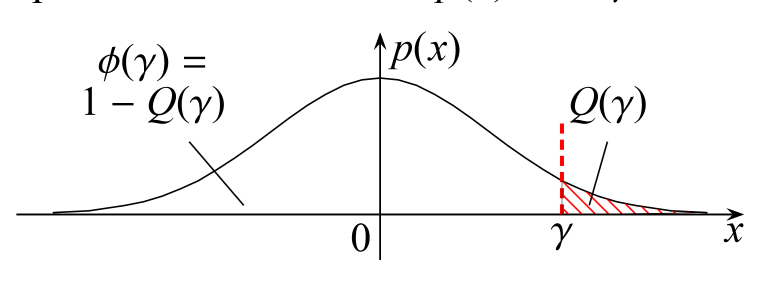
\includegraphics[width=0.10\textwidth]{Files/q.png}


    

    \section{Loss functions}
    Loss-Matrix $[l_{ij}]$ with $l_{ij} = l(\hat{\omega}=\omega_i, \omega=\omega_j) \geq 0$
    \subsubsection{0/1-Loss}
    \begin{math}
        l_{ij} =  \left\{\begin{array}{ll} 0 & i=j \\
                                           1 & i \neq j
                          \end{array}\right.
    \end{math}
    All errors are equally bad


    \vfill\null    % ugly fix to achieve formatting
    \columnbreak

    

    \section{Bayesian decision}
    \begin{tabular}{l|lllll}
               &                  MBR & \begin{tabular}[c]{@{}l@{}}MAP\\(BBR)\end{tabular}  & \begin{tabular}[c]{@{}l@{}}ML\\(BBR)\end{tabular}  & Minimax & \begin{tabular}[c]{@{}l@{}}Neyman-\\Pearson\end{tabular} \\ \hline
    data $\x$     &               \OK &  \OK    &  \OK  & \OK     & \OK            \\
    likelihood $p(\x|\omega_j)$ & \OK &   \OK  &  \OK  & \OK     & \OK            \\
    prior $P(\omega_j)$     &      \OK &  \YO  &  \YO  & \NO     & \NO            \\
    loss $l_{ij}$     &            \OK &   \OK &  \YO  & \OK     & \NO           \\
    % \OK: Bekannt &&&
    \end{tabular}\\
    \textcolor{blue}{predetermined}, \textcolor{lime}{known}, \textcolor{red}{unknown / varying}

    \subsection{Minimum Bayesian Risk (MBR)}
    Bayesian Risk: BR $= \sum_i \sum_j l_{ij}P_{ij} = E_{\hat{\omega},\omega} (l(\hat{\omega}, \omega)) $ \\
    $ = \int_{\mathbb{R}^d} \sum_{j=0}^1 l(\hat{H}(\x),H_j)\ p(\x,H_j)  \mathop{d\underline{x}} $ 

    \textcolor{red}{$ \hat{\omega}_{\textrm{MBR}}(\underline{x}) = \arg \min_{\hat{\omega}} R(\hat{\omega} \ | \ \underline{x}) $ \\
    with $ R(\hat{\omega}(\underline{x})=\omega_i \ | \ \underline{x}) = \sum_{j=1}^c l_{ij} P(\omega_j \ | \ \underline{x})  $ }\\

    \textbf{Likelihood ratio test:} 
    $\textrm{LR(T)}=\frac{p(\underline{x}  | \omega_1)}{p(\underline{x} | \omega_0)} \lessgtr^{\omega_0}_{\omega_1} = \frac{l_{10}-l_{00}}{l_{01}-l_{11}} \cdot \frac{p(\omega_0)}{p(\omega_1)} = \gamma$

    \textbf{Decision regions:}
    $R_0 = \{  x\ |\ \textrm{LR}(x) < \gamma  \}$,  $R_1 = \{  x\ |\ \textrm{LR}(x) > \gamma  \}$
    


    \subsection{MAP (maximum a posterior)}
    \textit{special case of MBR with 0/1-Loss}\\
    $\Rightarrow \  \textrm{BR} = \textrm{ER}$ \textit{error rate}\\
    $ \textrm{BR} = \sum\sum_{i\neq j}P_{ij}$

    $\hat{\omega}_{\textrm{MAP}} = \arg \max f_i(\x)$ \hspace{7pt} mit 
    $f_i(\x) = \ln p(\x | \omega_i)  + \ln P(\omega_i)$
    
    \textbf{Likelihood ratio test:} 
    $\frac{p(\underline{x}  | \omega_1)}{p(\underline{x} | \omega_0)} \lessgtr^{\omega_0}_{\omega_1} = \frac{p(\omega_0)}{p(\omega_1)} = \gamma_{\textrm{MAP}}$
    
    
    \subsection{ML (maximum likelihood)}
    \textit{special case of MAP with equal priors $P(\omega_i) = \frac{1}{c}$}\\
    balanced error rate: $ \textrm{BER} = \frac{1}{c} \sum\sum_{i\neq j} P(\hat{\omega}=\omega_i | \omega=\omega_j) P(\omega_j) $

    \textbf{Likelihood ratio test:} 
    $\frac{p(\underline{x}  | \omega_1)}{p(\underline{x} | \omega_0)} \lessgtr^{\omega_0}_{\omega_1} = 1 = \gamma_{\textrm{ML}}$

    
    \subsection{Minimax}
    Minimal expected error for ”pessimistic” (worst case) priors
    
    \subsection{Neyman-Pearson decision (NP) or CFAR}
    $ \textrm{LR} = \frac{p(\underline{x} \ |\ \omega_2)}{p(\underline{x} \ |\ \omega_1)} \lessgtr^{\omega_1}_{\omega_2} \gamma(\alpha)$ \\
    $\gamma$ determined by $P_{\textrm{FA}}= \int_{R_2(\gamma)} p(\underline{x} | \omega_1) \mathop{d\underline{x}} \stackrel{\textrm{!}}{=} \alpha$ bzw.
    $ P_{\textrm{FA}} = \int_{\hat{H}(\x)=H_1} p(\underline{x} | H_0) \mathop{d\underline{x}} $
    

    \vfill\null    % ugly fix to achieve formatting
    \columnbreak

    
    \section{Classifier}
    \subsection{Bayes plug-in}
    Naive Bayes plug-in: all features are independent (unlikely -> rough approx.)
    $\rightarrow p(\underline{x} | \omega_i) = \prod_{i=1}^d p(x_i | \omega_j \ ; \ \vartheta{ij})$


    \subsubsection{PDF estimation: parzen window}
    with \textbf{Gaussian Kernel} to estimate PDF:\\
    $\Phi(\underline{x})= \frac{1}{(2\pi)^{\frac{d}{2}}} e^{-\frac{1}{2}||x||^2}$ with $\mathcal{N}(0,\underline{I})$


    \subsection{SVM (support vector machine)}
    based on bin decision. Maximizes margin to sample.\\
    LDF $f(\x) = \underline{w}^T\x+w_0$\\
    Convex optimization problem (KKT)

    Multi-class via: one against one, hierarchical, (one against rest)

    \subsubsection{Hard Margin SVM}
    Binary dataset (1..N samples) linearly separable (hard margin) \\
    \underline{Primal problem:} $\min_{\underline{\omega},\omega_0} f(\underline{\omega},\omega_0) = \frac{1}{2} ||\underline{\omega}||^2$ s.t. $g_n(\underline{\omega},\omega_0) = 1 -y_n(\underline{\omega}^Tx_n + \omega_0) \quad 1\leq n\leq N$\\
    $\Rightarrow$ convex quadratic problem $\rightarrow$ KKT sufficient, strong duality\\

    \underline{Lagrange function:}
    $L(\underline{\omega}, \omega_0, \underline{\alpha}) = \frac{1}{2} ||\om||^2  +\sum_{n} \alpha_n g_n(\om, \omega_0) $\\
    $= \frac{1}{2} ||\om||^2  - \om^T \underline{\mathbf{X}} \underline{\alpha} - \omega_0 \underline{y}^T \underline{\alpha} + \underline{1}^T\underline{\alpha} $\\
    with $\underline{\mathbf{X}} = [y_1 \underline{x}_1,\ y_2 \underline{x}_2 ,\ ... ,\ y_N \underline{x}_N]$

    $\Rightarrow$ KKT conditions (4.5.4.3)\\
    Use dual problem to determine $\alpha_n$:\\
    $ d(\alpha) = -\frac{1}{2}\underline{\alpha}^T \mathbf{Q} \underline{\alpha} + \mathbf{1}^T \underline{\alpha} $, \hspace{3pt} $\mathbf{Q} = \mathbf{X}^T\mathbf{X}$
    
    with $\alpha_n$:\\
    $\om = \mathbf{X} \underline{\alpha} = \sum_{n\in \textrm{SV}} \alpha_n y_n \x_n $, \hspace{10pt}
    $\omega_0 = \frac{1}{|\textrm{SV}|}  \sum_{n\in \textrm{SV}} (y_n-\om^T\x_n) $

    Support-Vectors: all $\x_n$ with $\underline{\alpha_n}>0$ and must be on boundary ($g_n()  = 0$, but only sufficient)\\
    Only SV determien solution. 
    Use Dual problem to find $\alpha_n$

    \subsubsection{Soft Margin SVM}
    if not linearly seperable (even after feature mapping) \\
    Slack variable $\xi_n$: Optimization s.t.:\\
    $y_n(\underline{\omega}^Tx_n + \omega_0) \geq 1 +\xi_n $\\ 



    \subsection{Decision tree}
    Binary decision tree, not robust\\
    recursive splitting of dataset, can handle nominal (symbolic) features $\rightarrow$ nonmetric method.\\

    metric impurity $H(S_n)$ e.g. Gini-index: $H(S_n) = 1- \sum_{j=1}^c p_j^2$\\
    Search for biggest $\Delta H$ reduction

    Pruning: Cut subtrees with small impurity reduction (to avoid overfitting)
    

    \subsubsection{RF (Random forest)}
    many decision trees\\
    essemble method: combine models (with random samples of data/feature-set)

    

    \subsection{Overview}
    \begin{tabular}{l|lllll}
                              & kMeans & \begin{tabular}[c]{@{}l@{}}
                              nearest\\mean\end{tabular}
                                                  & NN & SVM & kNN \\ 
                                                      \hline
    supervised            &\NO     &\OK           &\OK &\OK  &\OK  \\
    multi-class           &\OK     &\OK           &\OK &\NO  &\OK  \\
    nonlinear dec. bound. &\NO     &\NO           &\OK &\NO  &\OK 
    \end{tabular}


    \vfill\null
    \columnbreak
    
    \section{Discriminant functions}
    learn discriminant functions from training samples $\rightarrow$ no pfd required

    \subsection{LDF (Linear discriminant functions)}
    decision boundaries are segments of hyperplanes
    $f_j(\underline{x})=\underline{\omega}_j^T\x+\omega_{j0}$

    
    \section{Features}
    
    \subsection{Feature mapping}
    e.g. polynomial mapping $f_i(\x) = w_{j0} + \sum_{k=1}^d w_{j,k} x_k +   \sum\sum_{k,l=1}^d w_{j,k,l} x_k x_l + ...$ 
    
    
    \subsection{Feature dimension reduction}
    to avoid overfitting: unknown parameters $\cdot 10 \ \approx \ N$ samples\\

    \subsection{Feature selection}
    - exhaustive search (often not possible)\\
    - single feature ranking (greedy algorithm - local min!)\\
    - Heuristics: e.g SFS, SSFS (sequential forward selection)
    
    \subsection{Feature transformation}
    LDA (linear discriminant analysis) uses Fisher ratio $F= \frac{|\sum_B|}{|\sum_W|}$

    \subsection{k-cross validation}
    \begin{minipage}{0.22\textwidth}
         $k-1$ folds per training, with median ER
    \end{minipage}
    \begin{minipage}{0.1\textwidth}
         \includegraphics[width=0.9\textwidth]{Files/k-fold.png}
    \end{minipage}

    \subsection{Hyperparameter optimization}
    \textit{e.g: type of classifier, kNN - number of k, GMM - number of models m, SVM - trade-off parameter $C$}\\
    additional validation-set needed.
    

    \section{KKT Condition}
    necessay conditions for local minimum:\\
    - stationarity: $\underline{\nabla}_{\x} L(\x^*, \underline{\alpha}^*, \underline{\lambda}^*) = 0$\\
    - primal feasibility: $g_i(\x^*) \leq 0$ and $h_i(\x^*)=0  \ \forall i$\\
    - dual feasibility: $\alpha^*_i \geq 0 \ \forall i $\\
    - complementary slackness: $\alpha^*_i g_i(\x^*) =  0 \ \forall i $\\

    \subsection{Primal and dual problem}
    primal problem $f^* = \min_{\x} f(\x)$ s.t. $g_i(\x) \leq 0 $ and $h_j(\x)=0$ (with $i=[1,p]$, $j=[1,q]$) \\
    can be converted to \textbf{dual problem:}
    $d^* = \max_{\underline{\alpha}, \underline{\lambda}} d(\underline{\alpha}, \underline{\lambda})$ s.t. $\alpha_i \geq 0 $\\
    $d(\underline{\alpha}, \underline{\lambda}) = \min_{\x} L(\x, \underline{\alpha}, \underline{\lambda})$
    
    convex primal problems: strong duality: $f^*=d^*$ (in general $d^*$ only lower bound for $f^*$)

\end{multicols}
\end{document}
